\begin{frame}{Vanishing and Exploding Gradients}
  \small
  \textbf{Backpropagation Through Time (BPTT)} spreads gradients across many time steps.
  
  \vspace{1em}
  {\color{red}\textbf{Vanishing Gradients:}}
  \begin{align*}
    \left\| \frac{\partial \mathcal{L}}{\partial h_t} \right\| \rightarrow 0
  \end{align*}
  \begin{itemize}
    \item[\textcolor{red}{$\blacktriangleright$}] Early layers barely learn
    \item[\textcolor{red}{$\blacktriangleright$}] Forget long-term dependencies
  \end{itemize}
  \vspace{0.5em}
  {\color{blue}\textbf{Exploding Gradients:}}
  \begin{align*}
    \left\| \frac{\partial \mathcal{L}}{\partial h_t} \right\| \rightarrow \infty
  \end{align*}
  \begin{itemize}
    \item[\textcolor{red}{$\blacktriangleright$}] Unstable updates, diverging weights
  \end{itemize}
\end{frame}

\begin{frame}{Solving for vanishing or exploding gradients}
  \begin{itemize}
    \item Identity RNN with ReLU activation
    \hfill
    \(
      \left[
        \begin{array}{ccccc}
          1 & 0 & 0 & 0 & 0 \\
          0 & 1 & 0 & 0 & 0 \\
          0 & 0 & 1 & 0 & 0 \\
          0 & 0 & 0 & 1 & 0 \\
          0 & 0 & 0 & 0 & 1 \\
        \end{array}
      \right]
    \)
    \item Gradient clipping
    \item Skip connections
      \begin{center}
        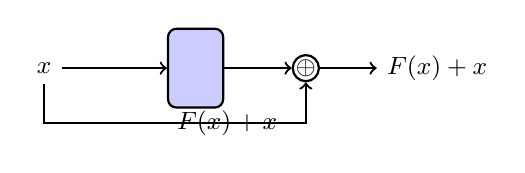
\begin{tikzpicture}[every node/.style={font=\small},thick,scale=1.0]
          % Nodes
          \node[left] (x) at (0,1) {$x$};
          \node[draw,rounded corners=3pt,fill=blue!20,minimum width=0.7cm,minimum height=1cm] (block) at (1.7,1) {};
          \node[circle,draw,inner sep=0pt,minimum size=0.3cm] (plus) at (3.1,1) {$\oplus$};
          \node[right] (out) at (4,1) {$F(x)+x$};
          
          % F(x)+x under skip arrow
          \node at (2.1,0.3) {$F(x)+x$};
          
          % Arrows: forward
          \draw[->,thick] (x) -- (block);
          \draw[->,thick] (block) -- (plus);
          \draw[->,thick] (plus) -- (out);

          % Skip connection
          \draw[->,thick] (x) |- (2.1,0.3) -| (plus);

        \end{tikzpicture}
      \end{center}
  \end{itemize}
\end{frame}

\begin{frame}{RNN tradeoffs}
  \textbf{RNN Advantages}
  \begin{itemize}
    \item Can process any length input.
    \item Computation for step t can (in theory) use information from many steps back.
    \item Model size doesn’t increase for longer input.
    \item Same weights applied on every timestep, so there is symmetry in how inputs
    are processed.
    \end{itemize}
    \textbf{RNN Disadvantages}
    \begin{itemize}
      \item Recurrent computation is slow
      \item In practice, difficult to access information from many steps back
      \end{itemize} 
\end{frame}
